\documentclass[a4paper,10pt, table]{/media/documents/Cours/Prof/Enseignements/tools/style/classDS}
\usepackage{/media/documents/Cours/Prof/Enseignements/2014_2015}

% Title Page
\titre{DM5}
% \seconde \premiereS \PSTMG \TSTMG
\classe{\premiereS}
\date{02 mars 2015}
%\duree{1 heure}
\sujet{1}
% DS DSCorr DM DMCorr Corr
\typedoc{DM}

\printanswers

\begin{document}

\maketitle

Le barème est donné à titre indicatif, il pourra être modifié. Vous rendrez le sujet avec la copie.

\begin{questions}

    \question
    Résoudre les équations suivantes
    
    
    \begin{eqnarray*}
        8 x^{  2 } + 5 x - 2 & > &0 \\
    \end{eqnarray*}

    \begin{solution}
        On commence par calculer le discriminant de $P(x) = 8 x^{  2 } + 5 x - 2$.
        \begin{eqnarray*}
            \Delta & = & b^2-4ac \\
            \Delta & = & 5^{  2 } - 4 \times 8 ( -2 ) \\ 
\Delta & = & 25 - 4 ( -16 ) \\ 
\Delta & = & 25 - ( -64 ) \\ 
\Delta & = & 89
        \end{eqnarray*}

        
        comme $\Delta = 89 > 0$ donc $P$ a deux racines

            \begin{eqnarray*}
                x_1 & = & \frac{-b - \sqrt{\Delta}}{2a} =  \frac{5 - \sqrt{89}}{2 \times 8} = -0.9 \\
                x_2 & = & \frac{-b + \sqrt{\Delta}}{2a} =  \frac{5 + \sqrt{89}}{2 \times 8} = 0.28
            \end{eqnarray*}


        
        Comme $a = 8$, on en déduit le tableau de signe de $P$
            \begin{center}
                \begin{tikzpicture}
                    \tkzTabInit[espcl=2]%
                    {$x$/1, $P$/2}%
                    {$-\infty$, -0.9 , 0.28 , $+\infty$}
                    \tkzTabLine{, +, z, -, z , +,}
                \end{tikzpicture}
            \end{center}
        On regarde maintenant où sont les $+$ dans le tableau de signe pour résoudre l'inéquation.
        \end{solution}

        \begin{eqnarray*}
            - 3 x^{  2 } + 2 x + 4 & \leq &0  \\
        \end{eqnarray*}
    \begin{solution}
        On commence par calculer le discriminant de $Q(x) = - 3 x^{  2 } + 2 x + 4$.
        \begin{eqnarray*}
            \Delta & = & b^2-4ac \\
            \Delta & = & 2^{  2 } - 4 ( -3 ) \times 4 \\ 
\Delta & = & 4 - 4 ( -12 ) \\ 
\Delta & = & 4 - ( -48 ) \\ 
\Delta & = & 52
        \end{eqnarray*}

        
            comme $\Delta = 52 > 0$ donc $Q$ a deux racines

            \begin{eqnarray*}
                x_1 & = & \frac{-b - \sqrt{\Delta}}{2a} =  \frac{2 - \sqrt{52}}{2 \times -3} = 1.54 \\
                x_2 & = & \frac{-b + \sqrt{\Delta}}{2a} =  \frac{2 + \sqrt{52}}{2 \times -3} = -0.87
            \end{eqnarray*}


        
        Comme $a = -3$, on en déduit le tableau de signe de $Q$
            \begin{center}
                \begin{tikzpicture}
                    \tkzTabInit[espcl=2]%
                    {$x$/1, $Q$/2}%
                    {$-\infty$, -0.87 , 1.54 , $+\infty$}
                    \tkzTabLine{, -, z, +, z , -,}
                \end{tikzpicture}
            \end{center}
        On regarde maintenant où sont les $-$ dans le tableau de signe pour résoudre l'inéquation.
        \end{solution}

        \begin{eqnarray*}
            8 x^{  2 } + 5 x - 2 & \geq & - 3 x^{  2 } + 2 x + 4 
        \end{eqnarray*}

        

        \begin{solution}
            On commence par se ramener à une équation de la forme $ax^2 + bx + c \geq 0$.
        \begin{eqnarray*}
            8 x^{  2 } + 5 x - 2 \geq - 3 x^{  2 } + 2 x + 4 & \Leftrightarrow & 8 x^{  2 } + 5 x - 2 - (- 3 x^{  2 } + 2 x + 4) \geq 0 \\
             & \Leftrightarrow & 8 x^{  2 } + 5 x - 2 - ( - 3 x^{  2 } + 2 x + 4 )\geq 0 \\ 
 & \Leftrightarrow & 8 x^{  2 } + 5 x - 2 + 3 x^{  2 } - 2 x - 4\geq 0 \\ 
 & \Leftrightarrow & ( 8 + 3 ) x^{  2 } + ( 5 + ( -2 ) ) x + ( -2 ) + ( -4 )\geq 0 \\ 
 & \Leftrightarrow & 11 x^{  2 } + 3 x - 6\geq 0
        \end{eqnarray*}

        

        Ensuite on étudie le signe de $R(X) = 11 x^{  2 } + 3 x - 6$.
        \begin{eqnarray*}
            \Delta & = & b^2-4ac \\
            \Delta & = & 3^{  2 } - 4 \times 11 ( -6 ) \\ 
\Delta & = & 9 - 4 ( -66 ) \\ 
\Delta & = & 9 - ( -264 ) \\ 
\Delta & = & 273
        \end{eqnarray*}

        
            comme $\Delta = 273 > 0$ donc $R$ a deux racines

            \begin{eqnarray*}
                x_1 & = & \frac{-b - \sqrt{\Delta}}{2a} =  \frac{3 - \sqrt{273}}{2 \times 11} = -0.89 \\
                x_2 & = & \frac{-b + \sqrt{\Delta}}{2a} =  \frac{3 + \sqrt{273}}{2 \times 11} = 0.61
            \end{eqnarray*}


        
        Comme $a = 11$, on en déduit le tableau de signe de $R$
            \begin{center}
                \begin{tikzpicture}
                    \tkzTabInit[espcl=2]%
                    {$x$/1, $R$/2}%
                    {$-\infty$, -0.89 , 0.61 , $+\infty$}
                    \tkzTabLine{, +, z, -, z , +,}
                \end{tikzpicture}
            \end{center}
        On regarde maintenant où sont les $+$ dans le tableau de signe pour résoudre l'inéquation.
            

        \end{solution}


    \question
    Tracer le tableau de variation des fonctions suivantes \textit{(Vous pouvez utiliser les nombres à virgules)}
    
    
    \begin{parts}
        \part $f:x\mapsto - 10 x^{  3 } + x^{  2 } - 7 x + 5$
        \begin{solution}
            Pour avoir les variations de $f$, il faut connaître le signe de sa dérivé. On dérive $P$
            
            \begin{eqnarray*}
                f'(x) & = & 3 ( -10 ) x^{  2 } + 2 \times 1 x + 1 ( -7 ) \\ 
f'(x) & = & - 30 x^{  2 } + 2 x - 7
            \end{eqnarray*}
            
            On étudie le signe de $P'$
            
            Ensuite on étudie le signe de $f'(x) = - 30 x^{  2 } + 2 x - 7$.
        \begin{eqnarray*}
            \Delta & = & b^2-4ac \\
            \Delta & = & 2^{  2 } - 4 ( -30 ) ( -7 ) \\ 
\Delta & = & 4 - 4 \times 210 \\ 
\Delta & = & 4 - 840 \\ 
\Delta & = & -836
        \end{eqnarray*}

        
        Alors $\Delta = -836 < 0$ donc $f'$ n'a pas de racine.

        
        Comme $a = -30$, on en déduit le tableau de signe de $f'$
            \begin{center}
                \begin{tikzpicture}
                    \tkzTabInit[espcl=2]%
                    {$x$/1, Signe de $f' $/2}%
                    {$-\infty$, $+\infty$}
                    \tkzTabLine{, -,}
                \end{tikzpicture}
            \end{center}

        \end{solution}

        
        
        \part $g:x\mapsto - 9 x^{  3 } - 8 x^{  2 } - 5 x - 2$

        \begin{solution}
            Pour avoir les variations de $g$, il faut connaître le signe de sa dérivé. On dérive $P$
            
            \begin{eqnarray*}
                g'(x) & = & 3 ( -9 ) x^{  2 } + 2 ( -8 ) x + 1 ( -5 ) \\ 
g'(x) & = & - 27 x^{  2 } - 16 x - 5
            \end{eqnarray*}
            
            On étudie le signe de $P'$
            
            Ensuite on étudie le signe de $g'(x) = - 27 x^{  2 } - 16 x - 5$.
        \begin{eqnarray*}
            \Delta & = & b^2-4ac \\
            \Delta & = & ( -16 )^{  2 } - 4 ( -27 ) ( -5 ) \\ 
\Delta & = & 256 - 4 \times 135 \\ 
\Delta & = & 256 - 540 \\ 
\Delta & = & -284
        \end{eqnarray*}

        
        Alors $\Delta = -284 < 0$ donc $g'$ n'a pas de racine.

        
        Comme $a = -27$, on en déduit le tableau de signe de $g'$
            \begin{center}
                \begin{tikzpicture}
                    \tkzTabInit[espcl=2]%
                    {$x$/1, Signe de $g' $/2}%
                    {$-\infty$, $+\infty$}
                    \tkzTabLine{, -,}
                \end{tikzpicture}
            \end{center}

        \end{solution}

        
        \part $h:x\mapsto - 7 x^{  2 } - 9 x + 3 - f(x)$

        
        

        \begin{solution}
            On commence par simplifier l'expression de $h$
            \begin{eqnarray*}
                h(x) & = & - 7 x^{  2 } - 9 x + 3 - f(x) \\
                h(x) & = & - 7 x^{  2 } - 9 x + 3 - ( - 10 x^{  3 } + x^{  2 } - 7 x + 5 ) \\ 
h(x) & = & - 7 x^{  2 } - 9 x + 3 + 10 x^{  3 } - x^{  2 } + 7 x - 5 \\ 
h(x) & = & 10 x^{  3 } + ( ( -7 ) + ( -1 ) ) x^{  2 } + ( ( -9 ) + 7 ) x + 3 + ( -5 ) \\ 
h(x) & = & 10 x^{  3 } - 8 x^{  2 } - 2 x - 2
            \end{eqnarray*}
            
        
            Pour avoir les variations de $h$, il faut connaître le signe de sa dérivé. On dérive $P$
            
            \begin{eqnarray*}
                h'(x) & = & 3 \times 10 x^{  2 } + 2 ( -8 ) x + 1 ( -2 ) \\ 
h'(x) & = & 30 x^{  2 } - 16 x - 2
            \end{eqnarray*}
            
            On étudie le signe de $P'$
            
            Ensuite on étudie le signe de $h'(x) = 30 x^{  2 } - 16 x - 2$.
        \begin{eqnarray*}
            \Delta & = & b^2-4ac \\
            \Delta & = & ( -16 )^{  2 } - 4 \times 30 ( -2 ) \\ 
\Delta & = & 256 - 4 ( -60 ) \\ 
\Delta & = & 256 - ( -240 ) \\ 
\Delta & = & 496
        \end{eqnarray*}

        
            comme $\Delta = 496 > 0$ donc $h'$ a deux racines

            \begin{eqnarray*}
                x_1 & = & \frac{-b - \sqrt{\Delta}}{2a} =  \frac{-16 - \sqrt{496}}{2 \times 30} = -0.1 \\
                x_2 & = & \frac{-b + \sqrt{\Delta}}{2a} =  \frac{-16 + \sqrt{496}}{2 \times 30} = 0.64
            \end{eqnarray*}


        
        Comme $a = 30$, on en déduit le tableau de signe de $h'$
            \begin{center}
                \begin{tikzpicture}
                    \tkzTabInit[espcl=2]%
                    {$x$/1, Signe de $h' $/2}%
                    {$-\infty$, -0.1 , 0.64 , $+\infty$}
                    \tkzTabLine{, +, z, -, z , +,}
                \end{tikzpicture}
            \end{center}

        \end{solution}
    \end{parts}

    \question
    Appliquer l'algorithme de tri vu en cours à la suite suivante
    \begin{center}
    \begin{tabular}{|*{6}{c|}}
        \hline
        6914 & 6851 & 6532 & 6884 & 6164 & 6495 \\
        \hline
    \end{tabular}
        
    \end{center}


\end{questions}
    
\end{document}

%%% Local Variables: 
%%% mode: latex
%%% TeX-master: "master"
%%% End:
